% Cap�tulo 2
\chapter{The Problem - Breakdown}

TODO: In this section we detail ...

\section{Problem Breakdown}
TODO: Breakdown each step of the problem.



\section{Proposed solution}

Service-Oriented Architecture (SOA) suggests that a Software Component can be seen as a set of sub-services. In the context of a Web Application, for example, it is possible to entirely replace a component just by changing the API address that it uses. This scenario of component replacement on cloud-based applications can be seen on (Figure~\ref{fig:apireplacement}).

\begin{figure}[ht!]
\centering
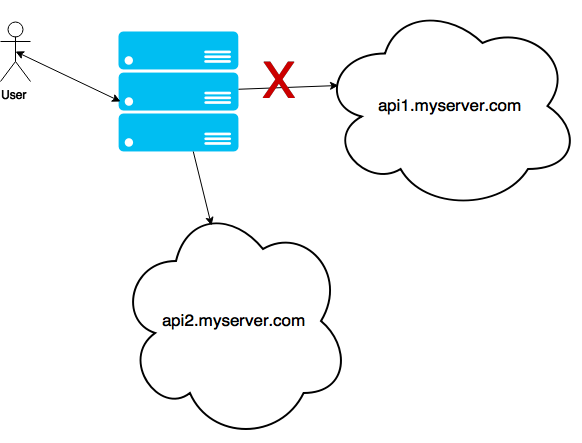
\includegraphics[width=100mm]{api.png}
\caption{Component replacement on cloud-based software.\label{fig:apireplacement}}
\end{figure}

As Section \ref{bibreview} presents, contributions can be made in the context of proposing SLA-Based and user-centered solutions to monitor component replacement scenarios.

In this work we assess the use of a SLA-Guided process to support the migration/replacement of relational databases with NoSQL ones. This process was developed and assessed with case studies.

The boundaries of this work could then be broadened to support the conception of a SLA-Guided process to support the migration/replacement of sotware components based on the cloud in future works.


\section{Roadmap}
%Detalhar l� em cima o que � PDCA
%nosso estudo vai ser baseado no PDCA, detalhado l� em cima, e pode ser dividido em 6 fases principais: 

To provide a better understanding of our work, we splitted the research in six main phases:

\begin{table}[!htb]
   \textsf{\caption{Work Phases.}} \label{tab:WorkPhasesTable}
   \centering
   \medskip
      \begin{tabular}{ | p{1cm}| p{2.5cm} | p {8cm} |}
   \hline
   Phase & Title & Description  \\ \hline
   1 & Identification of Case Studies \& SLAs  & On this step we aim to identify examples where a Database transition is needed or recommended in order to satisfy a SLA.
   We will try to work on production-ready and open-source softwares. If the complexity of these projects is too large for our scope, we will design and develop our own scenarios. \\ \hline
   2 & Plan & After the scenarios have been identified, we will propose architectural changes that could satisfy the SLA. These changes will be proposed by literature reviews and survey of industry experts.\\ \hline
   3 & Do & On this step we implement the architecture proposed on the previous step. \\ \hline
   4 & Check & On the check step we will verify if the proposed architecture and implementation satisfies the SLAs identified on the first step. \\ \hline
   5 & Act & Tweaks can be needed on the proposed architecture and implementation if the SLA is still not satisfied by the changes made on the previous step. On the act phase we investigate what else can be done to satisfy the SLA and refine the process defined on step 2. \\ \hline
   6 & Final Results & On the final step we aim to publish the results of our work on relevant database-related conferences and workshops. \\ \hline
   
   \end{tabular}
\end{table}





Each of these phases is composed by a number of steps, described below:
\begin{enumerate}
\item{Phase 1 - Identification of Case Studies \& SLAs }
\begin{enumerate}
\item {Step 1.1 - Scenario identification / Implementation: On this step we will search for open source projects and real-world scenarios where a Relational Database bottleneck has been identified. If the scope of these scenarios become too large, we will implement our own scenarios; }
\item {Step 1.2 - Identification of broken SLAs: We need to identify that the a set a constraints (i.e: execution time of a query) is not being met by the current architecture;}
\item {Step 1.3 - Implementation of ``runnable SLAs'' : On this step we will implement executable versions of the SLA identified on the previous step. These ``runnable SLAs" will be used to verify that a set of constraints is not being met by the current architecture. }
\item {Step 1.4 - Execution reports: After an executable SLA has been identified and implemented, execution reports will be consolidated to prove that the constraints of the SLA are being broken by the current architecture of the scenario.}

\end{enumerate}


\item{Phase 2 - Plan}
\begin{enumerate}
\item{Step 2.1 - Literature Review for each scenario: We will evaluate and search for solutions on how each scenario can make use of a NoSQL Database to meet the desired SLA; }
\item{Step 2.2 - Survey of industry experts: We will survey industry experts on how they would propose a NoSQL architecture to solve the problem described on each scenario. }
\end{enumerate}

\item{Phase 3 - Do}
\begin{enumerate}
\item{Step 3.1 - Planning of changes: We will gather the results from the previous phase and design the changes that will be performed on each scenario;}
\item{Step 3.2 - Implementation: We will implement the changes identified on the previous step. }
\end{enumerate}

\item{Phase 4 - Check}
\begin{enumerate}
\item {Step 4.1 - New Execution Reports: The same SLAs identified on the first step will be run on the modified scenarios, and execution reports will be consolidated.}
\item {Step 4.2 - Comparison of Results: The reports extracted on steps 4.1 and 1.4 will be compared to check if the changes made on Phase 3 satisfied the proposed SLA.}
\end{enumerate}

\item{Phase 5 - Act}
\begin{enumerate}
\item{Step 5.1 - Tweaks on the proposed architecture: If the SLA isn't being met yet, new changes might be needed, and on this step we join together the phases 2, 3 and 4 to iterate over the needed changes. }
\end{enumerate}


\item{Phase 6 - Final Results}
\begin{enumerate}
\item{Step 6.1 - Publish the results: We will submit the results of this study to academical conferences to have feedback from the community. }
\item{Step 6.2 - Write the final results: All the documents produced by our study and a final dissertation will be sent to the Universidade Federal do Rio Grande do Norte (UFRN).}


\section{Schedule}

A detailed view of the execution flow of our steps can be seen on Figure~\ref{fig:schedule}. 
\begin{figure}[ht!]
\centering
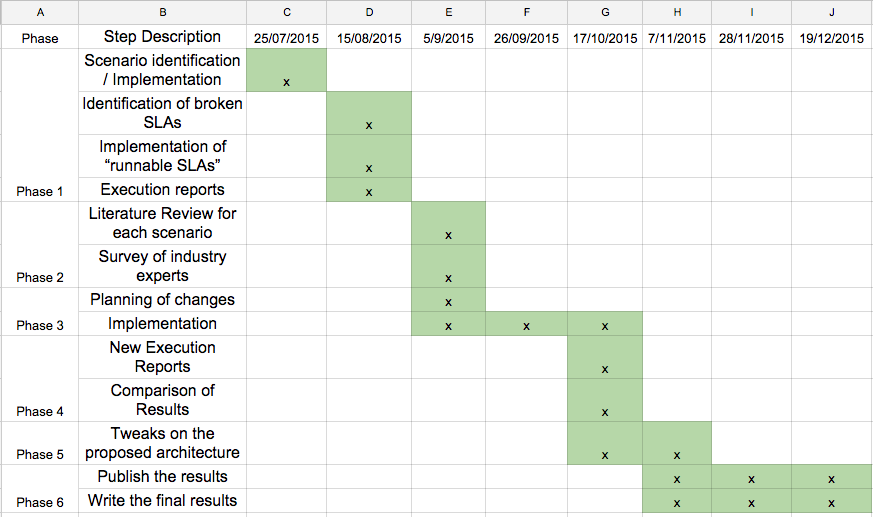
\includegraphics[width=140mm]{schedule.png}
\caption{Schedule.\label{fig:schedule}}
\end{figure}
\end{enumerate}

\end{enumerate}
